\chapter{Introduction}

\textbf{Note}: All project files can be found at \url{https://www.github.com/okayjustin/roborodentia2017} \


\section{Cal Poly Roborodentia}
The robot is designed to compete in the 2018 Cal Poly Roborodentia, the university's annual intramural robotics competition, and thus conforms to its particular specifications and requirements. Briefly, competitors must produce autonomous robots to collect and fire Nerf Rival Balls into nets to win points. A drawing of the field is shown below in Figure \ref{fig:roborodentia_field}. Two robots compete separately in each half so the effective field is a 4' wide by 8' long area enclosed by 4" walls. 1 inch PVC tubes along the 4' walls hold the balls which the robots fire into rectangular nets located along the 8' wall. The rules provide additional restrictions on robot dimensions, capabilities, and other aspects, to be covered specifically in the following chapters.

\begin{figure}[H]   % [h] means here
	\centering 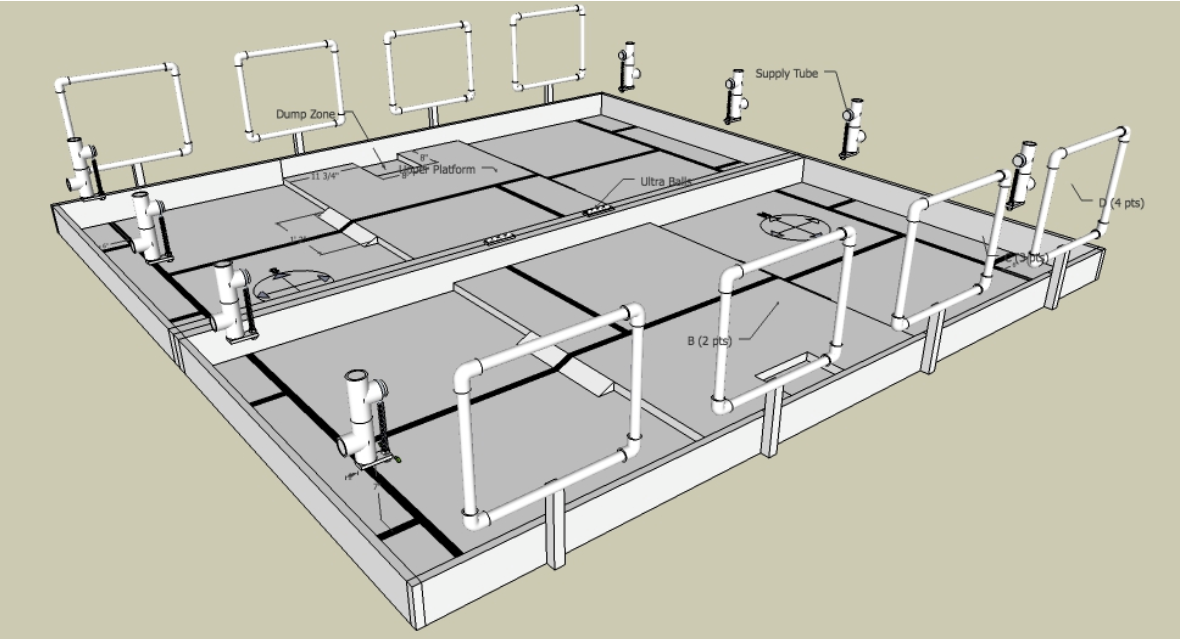
\includegraphics[width=6in, height=3.85in, keepaspectratio]{figures/roborodentia_field.png}
	\caption{Roborodentia Field \cite{roborodentia}}	\label{fig:roborodentia_field}
\end{figure}



